\documentclass[tikz,multi]{standalone}
\providecommand*{\xMin}{}%
\providecommand*{\xMax}{}%
\providecommand*{\yMin}{}%
\providecommand*{\yMax}{}%
\renewcommand*{\xMin}{0}%
\renewcommand*{\xMax}{4}%
\renewcommand*{\yMin}{0}%
\renewcommand*{\yMax}{4}%
\begin{document}
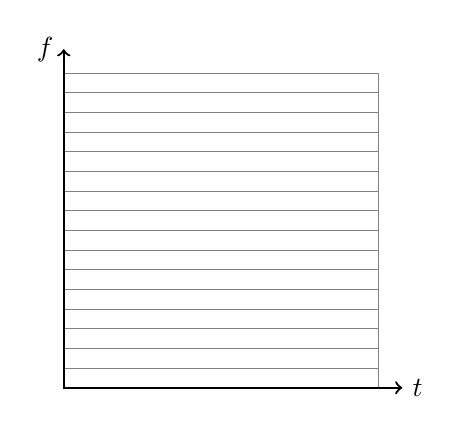
\begin{tikzpicture}
  \draw [very thin,gray] (\xMax,\yMin) -- (\xMax,\yMax)  node [below] at (\xMax,\yMin){};
  \foreach \i in {\yMin,...,3} {
    \foreach \j in {0,...,3} {
      \draw [very thin,gray] (\xMin,\i + \j/4) -- (\xMax,\i + \j/4) node [left] at (\xMin,\i + \j/4) {};
    }
  }
  \draw [very thin,gray] (\xMin,\yMax) -- (\xMax,\yMax) node [left] at (\xMin,\yMax) {};
  \draw [<->,thick] (\yMin,\yMax + 0.3) node (yaxis) [left] {$f$}
    |- (\xMax + 0.3,\xMin) node (xaxis) [right] {$t$};
\end{tikzpicture}
\end{document}
